\documentclass{article}
\usepackage{amsmath,amssymb,graphicx,tikz,standalone}
\usepackage{hyperref}
\title{CSC236 Winter 2015, Assignment 3}
\author{Connor Peet}
\renewcommand{\today}{~}
\hypersetup{pdfpagemode=Fullscreen,
  colorlinks=true,
  linkfileprefix={}}
\newcommand{\floor}[1]{\lfloor #1\rfloor}
\begin{document}
\maketitle

\begin{figure}
    \centering
    \documentclass{standalone}
\usepackage{tikz}
\begin{document}
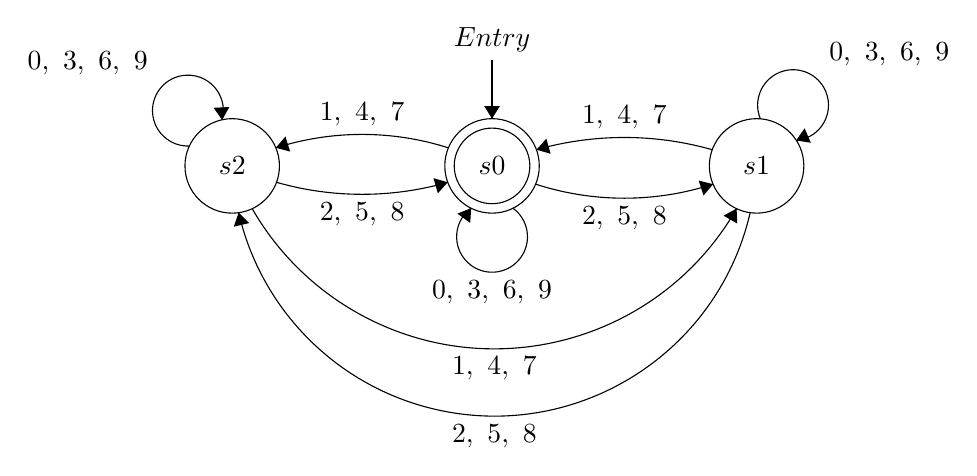
\begin{tikzpicture}[scale=0.2]
    \tikzstyle{every node}+=[inner sep=0pt]
    \draw [black] (33.2,-12.3) circle (3);
    \draw (33.2,-12.3) node {$s0$};
    \draw [black] (33.2,-12.3) circle (2.4);
    \draw [black] (50,-12.3) circle (3);
    \draw (50,-12.3) node {$s1$};
    \draw [black] (16.7,-12.3) circle (3);
    \draw (16.7,-12.3) node {$s2$};
    \draw [black] (33.2,-5.6) -- (33.2,-9.3);
    \draw (33.2,-5.1) node [above] {$Entry$};
    \fill [black] (33.2,-9.3) -- (33.7,-8.5) -- (32.7,-8.5);
    \draw [black] (47.236,-13.458) arc (-71.98994:-108.01006:18.229);
    \fill [black] (47.24,-13.46) -- (46.32,-13.23) -- (46.63,-14.18);
    \draw (41.6,-14.85) node [below] {${2,\mbox{ }5,\mbox{ }8}$};
    \draw [black] (36.015,-11.272) arc (105.8573:74.1427:20.438);
    \fill [black] (36.02,-11.27) -- (36.92,-11.53) -- (36.65,-10.57);
    \draw (41.6,-9.99) node [above] {${1,\mbox{ }4,\mbox{ }7}$};
    \draw [black] (50.245,-9.322) arc (203.03624:-84.96376:2.25);
    \draw (58.43,-6.01) node [above] {${0,\mbox{ }3,\mbox{ }6,\mbox{ }9}$};
    \fill [black] (52.51,-10.68) -- (53.44,-10.83) -- (53.05,-9.91);
    \draw [black] (19.469,-11.154) arc (107.71392:72.28608:18.015);
    \fill [black] (19.47,-11.15) -- (20.38,-11.39) -- (20.08,-10.43);
    \draw (24.95,-9.8) node [above] {${1,\mbox{ }4,\mbox{ }7}$};
    \draw [black] (30.39,-13.341) arc (-74.01892:-105.98108:19.757);
    \fill [black] (30.39,-13.34) -- (29.48,-13.08) -- (29.76,-14.04);
    \draw (24.95,-14.6) node [below] {${2,\mbox{ }5,\mbox{ }8}$};
    \draw [black] (48.731,-15.015) arc (-29.89393:-150.10607:17.742);
    \fill [black] (48.73,-15.01) -- (47.9,-15.46) -- (48.77,-15.96);
    \draw (33.35,-24.41) node [below] {${1,\mbox{ }4,\mbox{ }7}$};
    \draw [black] (49.591,-15.268) arc (-12.99968:-167.00032:16.668);
    \fill [black] (17.11,-15.27) -- (16.8,-16.16) -- (17.78,-15.93);
    \draw (33.35,-28.69) node [below] {${2,\mbox{ }5,\mbox{ }8}$};
    \draw [black] (34.523,-14.98) arc (54:-234:2.25);
    \draw (33.2,-19.55) node [below] {${0,\mbox{ }3,\mbox{ }6,\mbox{ }9}$};
    \fill [black] (31.88,-14.98) -- (31,-15.33) -- (31.81,-15.92);
    \draw [black] (13.993,-11.034) arc (272.65981:-15.34019:2.25);
    \draw (7.52,-6.53) node [above] {${0,\mbox{ }3,\mbox{ }6,\mbox{ }9}$};
    \fill [black] (16.06,-9.38) -- (16.52,-8.56) -- (15.52,-8.61);
\end{tikzpicture}
\end{document}

    \caption{DFA for question 1, which accepts a natural number string divisible by three}
    \label{fig:q1}
\end{figure}

\begin{figure}
    \centering
    \documentclass{standalone}
\usepackage{tikz}
\begin{document}
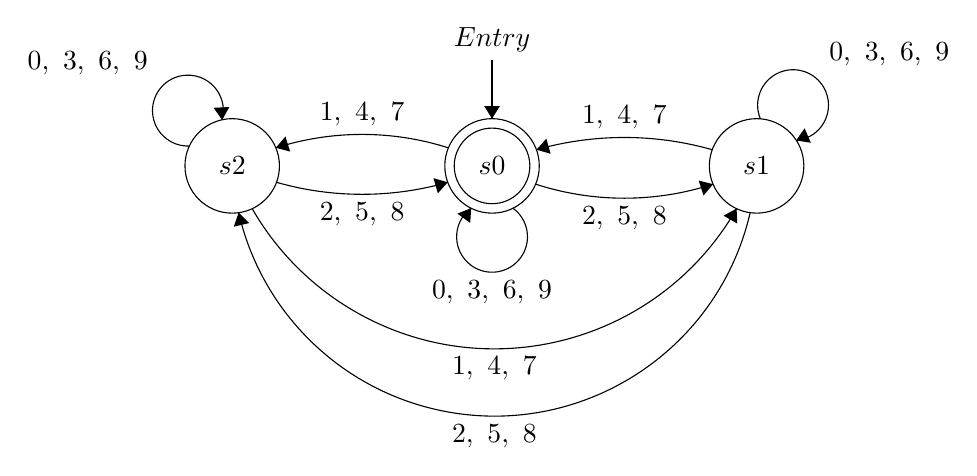
\begin{tikzpicture}[scale=0.2]
    \tikzstyle{every node}+=[inner sep=0pt]
    \draw [black] (33.2,-12.3) circle (3);
    \draw (33.2,-12.3) node {$s0$};
    \draw [black] (33.2,-12.3) circle (2.4);
    \draw [black] (50,-12.3) circle (3);
    \draw (50,-12.3) node {$s1$};
    \draw [black] (16.7,-12.3) circle (3);
    \draw (16.7,-12.3) node {$s2$};
    \draw [black] (33.2,-5.6) -- (33.2,-9.3);
    \draw (33.2,-5.1) node [above] {$Entry$};
    \fill [black] (33.2,-9.3) -- (33.7,-8.5) -- (32.7,-8.5);
    \draw [black] (47.236,-13.458) arc (-71.98994:-108.01006:18.229);
    \fill [black] (47.24,-13.46) -- (46.32,-13.23) -- (46.63,-14.18);
    \draw (41.6,-14.85) node [below] {${2,\mbox{ }5,\mbox{ }8}$};
    \draw [black] (36.015,-11.272) arc (105.8573:74.1427:20.438);
    \fill [black] (36.02,-11.27) -- (36.92,-11.53) -- (36.65,-10.57);
    \draw (41.6,-9.99) node [above] {${1,\mbox{ }4,\mbox{ }7}$};
    \draw [black] (50.245,-9.322) arc (203.03624:-84.96376:2.25);
    \draw (58.43,-6.01) node [above] {${0,\mbox{ }3,\mbox{ }6,\mbox{ }9}$};
    \fill [black] (52.51,-10.68) -- (53.44,-10.83) -- (53.05,-9.91);
    \draw [black] (19.469,-11.154) arc (107.71392:72.28608:18.015);
    \fill [black] (19.47,-11.15) -- (20.38,-11.39) -- (20.08,-10.43);
    \draw (24.95,-9.8) node [above] {${1,\mbox{ }4,\mbox{ }7}$};
    \draw [black] (30.39,-13.341) arc (-74.01892:-105.98108:19.757);
    \fill [black] (30.39,-13.34) -- (29.48,-13.08) -- (29.76,-14.04);
    \draw (24.95,-14.6) node [below] {${2,\mbox{ }5,\mbox{ }8}$};
    \draw [black] (48.731,-15.015) arc (-29.89393:-150.10607:17.742);
    \fill [black] (48.73,-15.01) -- (47.9,-15.46) -- (48.77,-15.96);
    \draw (33.35,-24.41) node [below] {${1,\mbox{ }4,\mbox{ }7}$};
    \draw [black] (49.591,-15.268) arc (-12.99968:-167.00032:16.668);
    \fill [black] (17.11,-15.27) -- (16.8,-16.16) -- (17.78,-15.93);
    \draw (33.35,-28.69) node [below] {${2,\mbox{ }5,\mbox{ }8}$};
    \draw [black] (34.523,-14.98) arc (54:-234:2.25);
    \draw (33.2,-19.55) node [below] {${0,\mbox{ }3,\mbox{ }6,\mbox{ }9}$};
    \fill [black] (31.88,-14.98) -- (31,-15.33) -- (31.81,-15.92);
    \draw [black] (13.993,-11.034) arc (272.65981:-15.34019:2.25);
    \draw (7.52,-6.53) node [above] {${0,\mbox{ }3,\mbox{ }6,\mbox{ }9}$};
    \fill [black] (16.06,-9.38) -- (16.52,-8.56) -- (15.52,-8.61);
\end{tikzpicture}
\end{document}

    \caption{DFA for question 2, which accepts any binary string containing a substring "1011"}
    \label{fig:q2}
\end{figure}

\begin{enumerate}

\item
    The DFA designed can be seen in Figure~\ref{fig:q1}. It has three states: $S_0$, $S_1$, and $S_2$. I will prove by contradiction that that is the minimum number of states required to fit the specification given in Question 1.

    Suppose we only have two states, and have some strings strings $w_1 = 2, w_2 = 22, w_3 = 222$. According to the specification, the empty string is accepted, so the initial state is accepting, and the other state must not accept. (Otherwise we'd just take any string, and that doesn't clearly work!) Therefore:

        \begin{itemize}
        \item $w_1$ must transition to the non-accepting state on $2$, since $2$ is not divisible by three.
        \item $w_2$ transitions to non-accepting on the first $2$ and must stay there on the seconds$2$, since $22$ is not divisible by three.
        \item $w_3$ causes a constradiction: it must transition to non-accepting on the first $2$, then accepting again on the next $2$, then it must \textit{stay} in accepting on the final $2$. However, it is required by other numbers that $2$ causes a transition \textit{out} of the accepting state.
        \end{itemize}

    Therefore, in order to build a DFA to specific we require at least three states.

\item
    The DFA designed can be seen in Figure~\ref{fig:q2}. It has five states. I will prove by contradiction that that is the minimum number of states required to fit the specification given in Question 1.

    Suppose we had four states, rather than five, and the strings $w_1 = \epsilon, w_2 = 1, w_3 = 10, w_4 = 101, w_5 = 1011$. Since there are five strings and four states, at least two of the strings must end up in the same state, and therefore be indistinguishable. However, for each string there is a \textit{unique} $n \in \mathbb{N}$ such that $\left\{w_xk_0\ldots k_n : k \in \left\{1, 0\right\}^*\right\} = 1011$. Therefore, any DFA with four states cannot be correct; it would either incorrectly accept or incorrectly reject at least one of the resultant strings.

\end{enumerate}

\end{document}
